\documentclass[tikz]{standalone}
\usetikzlibrary{calc}
\usepackage{pgfplots}
%\usepackage{khpreamble}
\usepgfplotslibrary{polar}
\pgfplotsset{compat=1.13}

\begin{document}
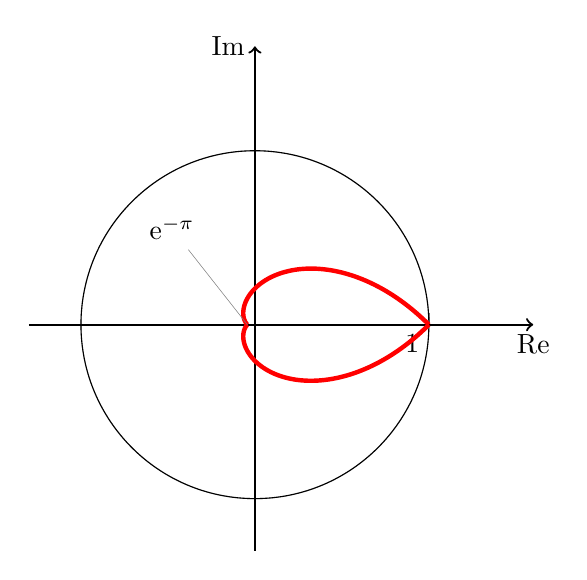
\begin{tikzpicture}[node distance=4cm]
\begin{polaraxis}[
   clip=false,
   width=6cm,
   height=6cm,
   xtick=\empty,
   %xticklabels={$ $, $\frac{\pi}{6}$, $\frac{\pi}{3}$, $ $, $\frac{2\pi}{3}$, $\frac{5\pi}{6}$, $ $, $\frac{7\pi}{6}$, $\frac{4\pi}{3}$, $ $, $\frac{5\pi}{3}$, $\frac{11\pi}{6}$},
   ytick={1},
   ymin=0, ymax=1,
   y tick label style={anchor=north east},
   %x coord trafo/.code=\pgfmathparse{#1+40},
   %y coord inv trafo/.code=\pgfmathparse{#1-40},
   %x dir=reverse,
   %xticklabel style={anchor=-\tick-90},
   %yticklabel style={anchor=east, xshift=-4.75cm},
   %y axis line style={yshift=-4.75cm},
   %ytick style={yshift=-4.75cm}
]
%\addplot+[domain=0:1, no markers, black, samples=800] (360*x,1); %
\draw[->, thick] (axis cs: 270, 1.3) -- (axis cs: 90, 1.6) node [left] {$\mathrm{Im}$};
\draw[->, thick] (axis cs: 180, 1.3) -- (axis cs: 0, 1.6) node [below] {$\mathrm{Re}$};

%\draw[-, ultra thick] (axis cs: 260, 2) -- (axis cs: 100, 2);

\addplot+[domain=0:1, no markers, red, ultra thick, samples=800] (180*x, exp(-pi*x); %
\addplot+[domain=0:1, no markers, red, ultra thick, samples=800] (-180*x, exp(-pi*x); %

\pgfmathsetmacro{\minexpi}{exp(-pi)}

\node[coordinate, pin={[pin distance=1.1cm] 120:{$\mathrm{e}^{-\pi}$}}] at (axis cs: 180, \minexpi ) {};

%\node[circle, fill, pin=-20:{$r$}, inner sep=0.5mm] at (axis cs: 30, 1) {};
\end{polaraxis}
\end{tikzpicture}
\end{document}
